


\documentclass[conference]{IEEEtran}

\usepackage{amssymb}
\setcounter{tocdepth}{3}
\usepackage{graphicx}
\usepackage{algorithm}
\usepackage{algpseudocode}
\usepackage{pifont}
\usepackage{array}

\begin{document}

\title{Concurrent Algorithms in SPIN Model Checker}

\author{\IEEEauthorblockN{M. Saqib Nawaz\IEEEauthorrefmark{1}, Hussam Ali\IEEEauthorrefmark{2} and M. IkramUllah Lali\IEEEauthorrefmark{3}} 
\IEEEauthorblockA{\IEEEauthorrefmark{1}Department of Information Science, School of Mathematical Sciences, Peking University, Beijing, China}
\IEEEauthorblockA{\IEEEauthorrefmark{2}Department of Computer Science, COMSATS Institute of Information Technology, Wah-Cantt, Pakistan}
\IEEEauthorblockA{\IEEEauthorrefmark{3}Department of Computer Science \& IT, University of Sargodha, Sargodha, Pakistan\\msaqibnawaz@pku.edu.cn,
hussamalics@gmail.com, drikramullah@uos.edu.pk}}

\maketitle

\begin{abstract}
Analysis and finding errors in concurrent software/system particularly when it is used in safety or industrial critical systems is gaining more 
and more attention. Software testing is an important technique for finding errors, however for concurrent algorithms, testing often does not ensure 
correctness or absence of errors. The model checker SPIN is widely and successfully used to formally verify the correctness requirements for systems
of concurrently executing processes. Software/system model is first developed in PROMELA modeling language and SPIN model checker accepts correctness
claims that are declared as linear temporal logic (LTL) formulas. In this article, two famous concurrent algorithms for mutual exclusion problem 
(Bakery algorithm and Dekker algorithm) are analyzed and formally verified in SPIN. Mutual exclusion for both algorithms is verified with in-line
assertion and as correctness claims with the help of LTL formulas. Furthermore, safety and liveness properties of both algorithms are verified 
with LTL formulas.
\end{abstract}

\begin{IEEEkeywords}
Bakery algorithm, Dekker algorithm, SPIN, LTL, PROMELA, Liveness, Safety.
\end{IEEEkeywords}
\IEEEpeerreviewmaketitle

\section{Introduction}
Formal methods offer rigorous mathematical frameworks that are used for the modeling and analysis of both hardware and software systems. Two popular 
frameworks in formal methods are \textit{model checking} and \textit{theorem proving} \cite{1}. Model checking approach was developed in early 1980's 
by Clarke and Emerson \cite{2}, Queille and Sifakis \cite{3}. System finite model is build first and state space of the model is exhaustively searched 
by the model checker to investigate whether a property holds in that model or not. Model checking approach is fast and automatic; sometimes it 
produces results in few minutes. Model checking can also be used to check specifications that are considered to be partial. Therefore, in case of 
system that has not been fully specified yet, model checking can give effective information related to the system correctness. 

Model checking suffers from the so called \textit{state-explosion problem} \cite{6}: systems state space grows prohibitively large with increase in 
the number of system variables and components. On the other hand, theorem provers have the ability to handle any system. Theorem provers are based 
on logics and offer a formal language for system modeling and an environment for mechanical reasoning and proofs \cite{5}. However, theorem provers 
are only partially automated and proof development can be hard and time consuming. If theorem prover fails to find any error, this does not 
necessarily mean that an error is present. It may be the case that user was unable to find the right proof. 

In this article, we have used SPIN \cite{7} model checker as it is well suited for the development and verification of concurrent and distributed 
systems. Other model checkers such as SLAM \cite{10} was originally build for verification of temporal safety properties in C programs
and BLAST \cite{4} for static analysis of C programs. However, SLAM and BLAST are widely used for the verification of device driver protocols.
KRONOS \cite{11} and UPPAAL \cite{12} are more suitable for real time systems verification and PRISM \cite{15} is used for modeling and analysis of 
systems with probabilistic behavior. Main focus in SPIN is on proving the correctness of process interactions. First, a model (in PROMELA) 
is developed that describes the system behavior. Correctness properties for the model are then specified for expressing the requirements on systems’ 
behavior. Finally, SPIN is run on the model for checking whether or not the desired properties hold in the model \cite{17}. In simulation mode, 
SPIN quickly evaluates different types of behavior of a system model. It also demonstrates those events (for fairness and starvation) that are 
rare to occur randomly. SPIN's graphical user interface, \textit{xSPIN} or \textit{iSPIN} can be used for the efficient visualization of 
simulation runs. In the verification mode, SPIN automatically inspects the whole state space of the model and look for a counterexample. 
A counterexample is an incorrect computation that violates a correctness specification. If SPIN detects any counterexamples then these incorrect 
computations can be investigated in detail in the interactive simulator in order to find and correct the computation. 

System models in SPIN are described in PROMELA (a Process Meta Language) \cite{17} and linear temporal logic (LTL) is used for expressing 
requirements properties that are later verified in SPIN. The syntax and semantics of PROMELA expressions is similar to C/C++. The control statements
used in PROMELA are taken from a formalism known as \textit{guarded commands} invented by Dijkstra \cite{23}. This formalism is well suited to 
express nondeterministic behavior. Therefore, PROMELA language is used to find good abstractions of system design. Main focus in PROMELA is on 
modeling of process synchronization and coordination among them. Puneli \cite{16} suggested temporal logic as a suitable formalism for concurrent 
programs. One of the advantages of using LTL formula is that it can be converted into a B\"{u}chi automaton \cite{24} and SPIN mechanically converts
LTL formula to B\"{u}chi automata. Generated automata by SPIN only accept those system executions where the corresponding LTL formula is 
satisfied. Correctness claims in SPIN are generally used for formalizing spurious behaviors of system, such as unwanted behaviors. 
LTL formula can also be used for such claims by changing positive LTL formula into a negative one with the help of logical negation operator.

It is generally acknowledged that increasing the number of transistors in processor does not enhance the computing capability of a system due
to physical limitation in modern processor designs. This limitation has led to the development of multi-core processors [20, 22]. In order to 
utilize multi-core processors, increased attention is given to algorithms that achieve maximal concurrency for high performance. Concurrent
programming provides a framework to effectively use parallel, structure and distributed systems that execute different simultaneous tasks at a 
time. However, the unpredictable interaction among concurrently running processes may cause software defects which are hard to find. While program 
verification remains desirable, the advent of concurrent programming has made program verification both more necessary and more difficult. 
Dijkstra \cite{8} first proposed the solution for the problem that concurrently running processes may require restricted access to resources that are 
shared among different processes. The problem is called as mutual exclusion in \cite{9}. 

In mutual exclusion problem, several processes say \textit{N} communicate through shared variables and these processes repeatedly make attempts 
to access a shared resource.

 \textbf{process (N) =}\\
 \hspace*{.5cm}\textbf{begin loop}\\
 \hspace*{.6cm}\textit{Non Critical Section};\\
 \hspace*{.7cm}Entry; \textit{Critical Section}; Exit;\\
\hspace*{.6cm}\textit{Non Critical Section};\\
\hspace*{.5cm}\textbf{end loop}\\

 The PROMELA code for simple mutual exclusion problem for \textit{N} processes and its corresponding transition system is shown in Fig. 1. 
 The construct \textit{proctype} is used for declaring the behavior of process. Here, \textit{N} (\textit{N}  is a constant) instances of 
 \textit{proctype} is activated in initial system state. 
 A \textit{bool} type variable CS is declared (\textit{line 1}) that is set to 1 (\textit{true}) by a process before entering critical section 
 (\textit{line 3}) and reset to 0 (\textit{false}) after process leaves the critical section (\textit{line 5}).
\begin{figure}[!ht]
{\small 
\begin{verbatim}
  1 bool CS = false;
  2 active [N] proctype P(){
  3 NCS: //Non Critical Section 
  4 Entry: CS = true; //Critical Section
  5 Exit: CS = false;
  6 goto NCS: }      
\end{verbatim}}\vspace{-3mm}
\centering\includegraphics[width=0.22\textwidth]{11}
\caption{PROMELA code for mutual exclusion problem and resultant transition system generated by SPIN} 
\end{figure}

In mutual exclusion problem, \textit{Non Critical Section} (NCS) and \textit{Critical Section} (CS) are program fragments. 
The problem is to device \textit{Entry} and \textit{Exit} in such a way that following holds: 
\begin{itemize}
 \item Mutual exclusion: Total number of processes in CS should remain $\leq$ 1.
 \item Progress requirement: If some process enters Entry, then eventually some process will enter CS. 
 \item Freedom from starvation requirement: If some process enters Entry, then eventually that process will enter CS. 
\end{itemize}

Among the proposed algorithms for mutual exclusion, Bakery algorithm \cite{13} and Dekker algorithm \cite{9} stands out because of their simplicity
and elegance. 
The goal in this work is to use SPIN to analyze and formally verify the Bakery algorithm and Dekker algorithm. The rest of the article 
consists of two main parts. In first part (Section II), Bakery algorithm for \emph{N} processes is first modeled in PROMELA. Correctness properties 
of Bakery algorithm are expressed in LTL syntax. Designed model of Bakery algorithm in PROMELA and its properties are then verified through SPIN.
In second part (Section III), modeling of generalized Dekker algorithm and its verification in SPIN is carried out along with verification of 
its properties. Article concludes with some remarks in Conclusion (Section IV).

\section{Bakery Algorithm in SPIN}
Bakery algorithm \cite{13} offers a simple solution for the mutual exclusion problem without depending on any form of central control such 
as semaphores. Furthermore, Bakery algorithm allows the processes to continue their operation despite the failure of any individual process. 
Bakery algorithm working is similar to the way customers get their turns in bakeries by drawing a number from a machine and the baker served the 
customer with the lowest number. Bakery algorithm for \textit{N} processes is listed in Fig. 2.
\begin{figure}[!ht]
\hspace{0.2cm}\textbf{Process P(i)};\\
\hspace*{0.3cm}non critical section;\\
\hspace*{0.3cm}L1: choosing[i] := 1;\\
\hspace*{0.4cm}num[i] : = 1 + max(num[1], ..., num[N]);\\
\hspace*{0.4cm}choosing[i] := 0;\\
 \hspace*{0.4cm}\textbf{for j in 1...N step 1 do}\\
\hspace*{0.5cm}\textbf{begin}\\
\hspace*{0.5cm}L2: \textbf{if} choosing[j] $\neq$ 0 then \textbf{goto} L2;\\
\hspace*{0.5cm}L3: \textbf{if} num[j] $\neq$ 0 and (num[j]) $<$ (num[i]) then \textbf{goto} L3;\\
\hspace*{0.5cm}end;\\
\hspace*{0.4cm}critical section;\\
\hspace*{0.4cm}num[i] : = 0;\\
\hspace*{0.4cm}non critical section;\\
\hspace*{0.4cm}\textbf{goto} L1;\\
\hspace*{0.2cm}\textbf{end}
\caption{Bakery algorithm \cite{13}}
\end{figure}

Each process in Bakery algorithm contains a part of CS and this part cannot execute concurrently with the CS parts of other processes. 
If a process shows interest to enter its CS, it will receive a number in NCS and the process with the lowest number is allowed to enter its CS. 
In SPIN, checking Bakery algorithm for arbitrary number of process is impossible as the drawn numbers are unbounded which will lead to an infinite 
state space. However, modifications have been done for restricting the drawn numbers that will lead to a finite state space. Baier and Katoen 
\cite{33} developed a model for Bakery algorithm for 2 customers (processes). Dedic and Meolic \cite{19} formally modeled three versions of Bakery
algorithm for two processes using process algebra. Properties of developed models are expressed in action computation tree logic (ACTL) \cite{21}, 
and model checker is used for the verification of ACTL formulas. Moreover, Hesselink \cite{34} formally verified Bakery algorithm in theorem prover 
PVS. We have developed a model for Bakery algorithm in PROMELA for \emph{N} processes. The complete verification model of Bakery algorithm in 
PROMELA is included in Appendix A. The transition system for Bakery model generated by SPIN is shown in Fig. 3.\vspace{-4mm}
\begin{figure}[!ht]
\centering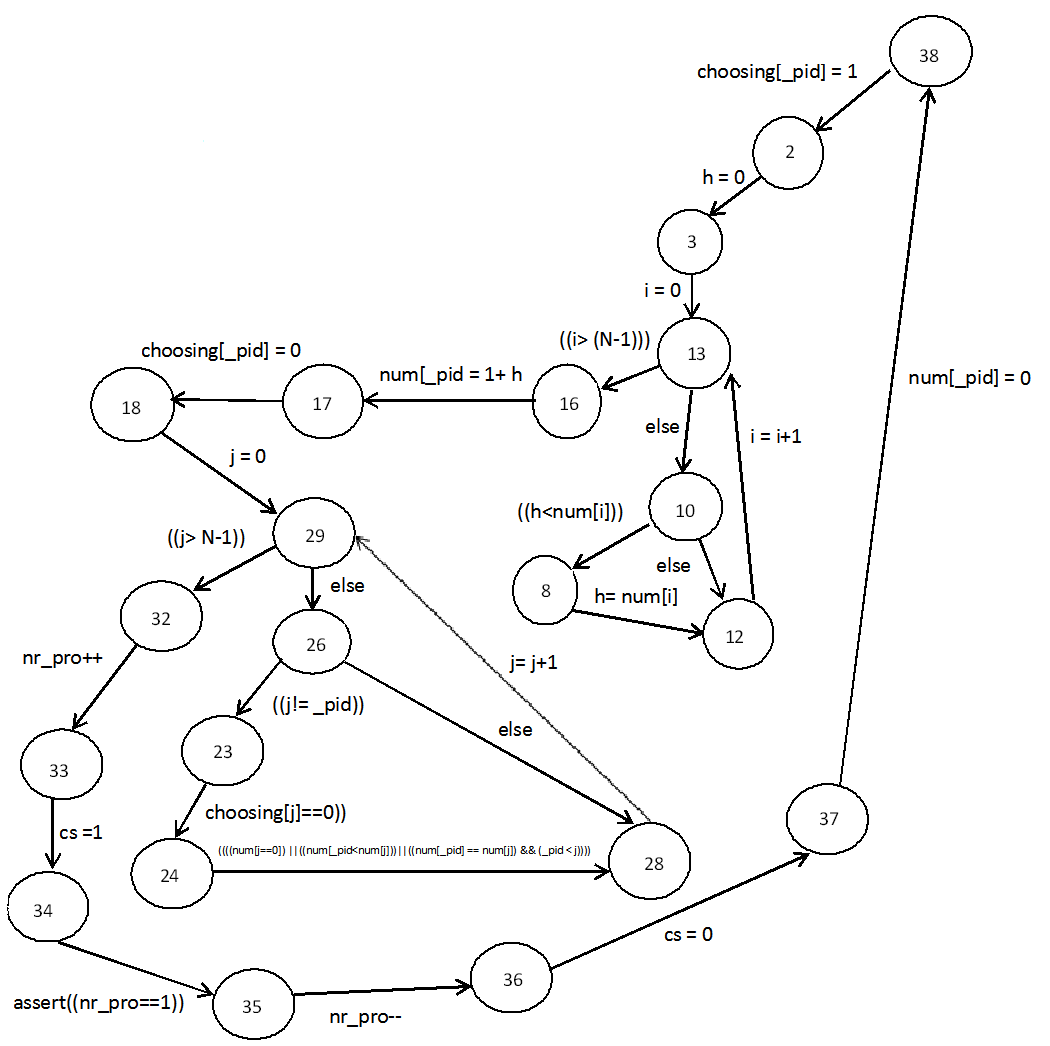
\includegraphics[width=0.45\textwidth]{bakerymodel}
\caption{Labeled transition system for Bakery algorithm} 
\end{figure}

In PROMELA code, there is one asynchronously executing process $P$, which repeatedly makes call on again ($line$ $6$ in Appendix A) routine. 
In PROMELA model, each process chooses its own number ($line$ $9$) which is modeled by a $bool$ variable $choosing[N]$ ($line$ $2$). Before 
entering CS part,
each process gets a ticket number ($line$ $19$). After leaving CS, each process gets number 0 ($line$ $37$), which shows that the process is no more 
interested in accessing the CS.

To get a first glimpse of the complexity of Bakery model, an exhaustive verification with SPIN is done to prove some of the default 
safety properties that include deadlock absence, race conditions and unreachable code. The Bakery model is run with the default options for memory
management and reduction techniques to measure the state space size that the SPIN verifier creates for proof completion. Verification results for 
different number of processes are shown in Table I.
\begin{table}[!ht] \label{t1}
\caption{Complexity increases with total number of processes}
\centering
 \begin{tabular}{|>{\centering}p{1.6cm}|>{\centering} p{1.6cm} |>{\centering} p{1.8cm} |>{\centering} p{1.6cm}|}
\hline
\textbf{Number of Processes} & \textbf{Total no. of States} & \textbf{Memory used (in MB)} & \textbf{Time (in Sec)}\tabularnewline
\hline
2 & 178713 & 69.910 & 0.06\tabularnewline
3 & 22862669 & 1023.914 & 15\tabularnewline
4 & 30541985 & 1571.375 & 461\tabularnewline
5 & X & X & X\tabularnewline
\hline
\end{tabular}  
X:Verification cannot be completed on system with 2GB memory\end{table}

It is clear from Table I that the state space for the model, memory and time required by SPIN for verification increases with increase in the total 
number of processes. We have performed the verification runs on Core i5 system with 4GB RAM. Bakery model can be verified for more than 4 processes
on systems with higher memory.

For the formal verification of concurrent programs, safety and liveness properties are of primary importance and these two properties 
have been studied extensively. For verification, SPIN generates the state space of a program and then it searches for a counterexample 
(if one exists) to the correctness specification. We can use the construct $assertion$ for correction specification inside PROMELA model. 
$Assertion$ statement is also used to express simple safety properties. This statement can be added between any two statements of a 
program and if SPIN finds a single computation during the search of state space that leads to a false $assertion$, it means that either the 
developed model is incorrect or the assertion is unable to properly express the correctness property for that model. Note that a computation
represents a sequence of states that starts with initial state and continue with the states that occur as each statement in the model is 
executed. Mutual exclusion property is proved by inserting an in-line $assertion$ to the PROMELA model, $assert(nr\_pro$ $==$ $1$) ($line$ $35$).
\emph{Assertion} is added at the point where a process is in its CS. 

However, $assertions$ are added at a specific control in the model so it can be used for specifying limited correctness properties. 
Generally, it is required to express a correctness property that does not depend on specific control points. Furthermore, $assertion$ fails 
to express some properties as the property cannot be checked by evaluation of an expression in a single state of computation. For example in
mutual exclusion problem, consider the two properties (absence of deadlock and absence of starvation) that can be represented by means of a 
relation between two computation states: a state $s$ where a process intends to enter CS and another state $t$ where process does enter CS. In this 
case, state $t$ may occur hundred (or even thousands) of states later than state $s$ in the computation. 

Such properties can be expressed in SPIN with a finite automaton known as never claim that is executed together with automaton generated from 
the PROMELA. However, specifying a correctness property as a never claim is hard. SPIN can automatically translate a property written as LTL 
formula into a never claim.  LTL is based on propositional calculus and LTL formula is made from atomic proposition combined with operators of 
propositional calculus and temporal operators that are listed in Table II.
\begin{table}[!ht]
\caption{Propositional Calculus and Temporal Operators in PROMELA}
\centering
 \begin{tabular}{|>{\centering}p{2.5cm}|>{\centering} p{2cm} |>{\centering} p{2cm} |}
 \hline
\textbf{Propositional Calculus Operators} & \textbf{Math Symbol} & \textbf{SPIN Symbol}\tabularnewline
\hline
Not & $\neg$ & !\tabularnewline
And & $\land$ & \&\&\tabularnewline
Or & $\lor$ &$||$\tabularnewline
Implies & $\rightarrow$ & $->$\tabularnewline
Equivalent & $\leftrightarrow$ & $<->$\tabularnewline
\hline
\textbf{Temporal Operators} & \textbf{Math Symbol} & \textbf{SPIN Symbol}\tabularnewline
\hline
Always & $\square$ & [ ]\tabularnewline
Eventually & $\diamond$ & $<>$\tabularnewline
Until & $\cup$ & U\tabularnewline
\hline
\end{tabular}    
\end{table}

The $\square$ and $\diamond$  temporal operators in Table II are unary, whereas $\cup$ is a binary operator. 
LTL formula can be used in PROMELA to express both the safety and liveness properties of a system as a global property. 

\subsection{Safety Properties}
Safety is typically described as those set of properties that the system should not violate. Therefore, 
safety defines the bad things that should be avoided \cite{17}. Formal definition of safety properties is: \\
\textbf{Definition 1.} Let \emph{F} represents an LTL formula and a computation is represented as \emph{C} 
= ($s_0$, $s_1$, $s_2$,...). Then $\square$\emph{F} (read as always $F$) is \emph{true} in state $s_j$ iff \emph{F} is \emph{true} $\forall$ 
$s_j$ in $C$ such that $j$ $\geq$ $i$.

Formula $\square$\emph{F} is a safety property as it shows that the computation is safe in a sense that only `good' things will happen and `bad' 
things will never happen. To prove that mutual exclusion holds in the Bakery model, we defined the following:  

\begin{verbatim}
     # define_mutex (nr_pro <= 1)
\end{verbatim}

LTL formula \emph{![]mutex} is checked in SPIN. Negation on the formula expresses the existence of a computation where total number of process in 
CS is greater than 1. Generated never claim and its corresponding B\"uchi automaton is shown in Fig. 4.

\begin{figure}[!ht]
{\small \begin{verbatim}
 never { /* ![]mutex */
  T0_init:
   do
     ::atomic{!(mutex)-> assert(!(!(mutex)))}
     ::(1)-> goto TO_init
   od;
 accept_all:
  skip }
\end{verbatim}}\vspace{-5mm}
\centering\includegraphics[width=0.2\textwidth]{13}
\caption{Never claim and corresponding B\"uchi automaton} 
\end{figure}

For verification of generated never claim, SPIN generates a B\"uchi automaton by computing the synchronous product of automaton for the model 
and the B\"uchi automaton for never claim. If the resulted B\"uchi automaton accepts empty language then the correctness claim is not 
satisfied by the model. However, if the accepted language is nonempty then the language contains those system behaviors that satisfy the 
corresponding LTL formula. The entire computation is done by SPIN using nested depth first search (DFS) algorithm \cite{25}. Nested DFS algorithm 
terminates in case an acceptance cycle is found that represents a counterexample to the never claim or in case when the overall product has been
computed. In later case, no counterexample exists for the never claim. The working of nested DFS algorithm in SPIN is explained in \cite{26}. 
Along-with nested DFS algorithm, SPIN used several other optimization algorithms in order to make verification runs more effective, it includes:
\begin{itemize}
 \item Partial order reduction \cite{27},
 \item Bit-state hashing (Memory management) \cite{28},
 \item State vector compression (Memory management) \cite{29},
 \item Minimized automaton encoding of states \cite{30}, and
 \item Slicing algorithm \cite{31}.
 %\item Parallel DFS Algorithm \cite{35},
\end{itemize}

Mutual exclusion is also proved with LTL formula \emph{\{[] ((P@CS) $->$ (nr\_pro==1))\}}.

\subsection{Liveness Property}
Liveness represents those set of properties that the system must satisfy. Liveness also defines the good things that capture the 
required functionality of a system \cite{7}. Liveness properties can be formally defined as:\\
\textbf{Definition 2}. Let \emph{F} represents an LTL formula and a computation is represented as \emph{C} = $(s_0, s_1, s_2,...)$. 
Then $\diamond$\emph{F} (read as eventually \emph{F}) is \emph{true} in state $s_j$ iff \emph{F} is \emph{true} for some $s_j$ in \emph{C} such that 
$j$ $\geq$ $i$.

Formula $\diamond$\emph{F} is a liveness property as it shows that eventually something good will happen. For Bakery algorithm, a liveness property 
can be: If any process shows interest to enter its CS, then that process will eventually access its CS. This property is proved with 
formula \emph{\{P[1]@again  $-> <>$ P[1]@CS}\}. This property can also be proved by adding a \emph{Boolean} variable \emph{cs} to the code.
{\small \begin{verbatim}
  34  nr_pro++;
  35  cs = true;
  36  CS: assert(nr_pro==1)
  37  nr_pro--;
  38  cs = flase; 
\end{verbatim}}

Variable \emph{cs} is used in formula \emph{ltl b1 \{$<>$cs\}}. Similarly, initially some process may have no interest to enter CS but it shows 
interest after some time. We have proved this latching property with formula \emph{ltl b2 \{$<>[$ $]$ ((P[3]\@again) $->$ (p[3]\@CS))\}}. Formula 
\emph{b2} ensures that if a process say process 3 shows its interest for CS, eventually process 3 will always get a chance to enter its CS. 
Absence of starvation is proved with \emph{ltl b3 \{ $[$ $]<>$ ((P[3]@again) $->$ (P[3]@CS))\}}. This formula also expresses the property that 
formula \emph{F} is \emph{true} infinitely often. It is important to note that a counterexample for safety property consist of one state where the 
formula evaluates to false which shows that something ‘bad’ has happened. On the other hand, a counterexample for liveness property consists 
of an (infinite) computation which shows that something ‘good’ never happened.

\section{Dekker Algorithm in SPIN}
Dekker first proposed the mutual exclusion problem and Dijkstra \cite{8} give the first solution to the mutual exclusion problem for two processes 
and attributed the proposed solution to Dekker. Dekker algorithm for arbitrary number of processes were presented and proved in [8, 9]. 
In Dekker algorithm for two processes, behavior of both the processes is same. Process say $p_1$, for example, show its interest for the CS
by setting its variable $(x_1)$ to \emph{true}. Process $p_1$ then tests $x_2$ (variable of process say $p_2$) to check whether second 
process $p_2$ is interested in the CS. If $p_2$ is not interested, then $p_1$ enters its CS. If $p_2$ is interested, 
then $p_1$ sets its variable to \emph{false} and tries again. Same is also the case for process $p_2$. Due to the same behavior of both processes, 
a form of deadlock known as \emph{after-you-after-you} may occur. In this kind of deadlock, both processes are trying to enter 
their CS and keep withdrawing at the same time. This deadlock can be avoided by adding a shared variable \emph{turn} that can be 
either 1 or 2. \emph{Turn} variable is used to give priority to a process. When a process wants to leave its CS, it will change 
the value of \emph{turn} to \emph{false}. 

Martin \cite{14} proposed a new generalization of Dekker algorithm for \emph{N} processes. Proposed Dekker algorithm for \emph{N} processes is listed 
in Fig. 5.
\begin{figure}[!ht]
\hspace{.2cm}\textbf{Process P(i)};\\
\hspace*{.3cm}non critical section\\
\hspace*{.3cm}L1: n(i) := true;\\
\hspace*{.4cm}\textbf{for j in 1...N step 1 do}\\
\hspace*{.5cm}\textbf{begin}\\
\hspace*{.6cm}\textbf{if} [(j $\neq$ i and n[j] =  true) $\rightarrow$ n(i) := false;\\
\hspace*{4cm}(turn = 0 $\lor$ turn = i)\\
\hspace*{.6cm}turn := i;\\
\hspace*{.6cm}n(i) := true ];\\
\hspace*{.5cm}\textbf{end};\\
\hspace*{.3cm} critical section\\
\hspace*{.3cm}n(i) := false;\\
\hspace*{.3cm}turn := 0;\\
\hspace*{.3cm}non critical section\\
\hspace*{.3cm}\textbf{goto} L1\\
\hspace*{.2cm}\textbf{end}
\caption{Generalized Dekker algorithm for N processes}
\end{figure}

The specification of Dekker algorithm in PROMELA is shown in Appendix B. 
\begin{figure}[!ht]
\centering\includegraphics[width=0.3\textwidth]{dekkermodel}
\caption{Labeled transition system for Dekker algorithm} 
\end{figure}

In Process $p(i)$, $1 \leq i \leq N$ , where $N$ represent the total number of processes. Each process uses its bool variable $n(i)$ to declare 
its interest to enter the CS. In Dekker model, one asynchronously executing process $P$ repeatedly makes call on again ($line$ $6$) routine. 
If a process $i$ wants to enter its CS then it sets $n(i)$ to $true$ ($line$ $9$). Checking of interest of other processes is done by testing 
in the \emph{do loop}. If other process has interest to enter its CS then process $i$ withdraw its candidacy by setting $n(i)$ to $false$ ($line$ $14$). 
Global variable $turn$ is declared ($line$ $2$) that is used in the same way as in Dekker's first solution. When a process wants to leave CS, 
it sets the value of $n(i)$ to $false$ ($line$ $26$). Fig. 6 shows the transition system for Dekker model.

\subsection{Verification Results}
During verification of basic properties of Dekker model, the total number of state space that is explored, memory used and the elapsed time by 
SPIN for different number of processes is shown in Table III. Verification was completed in less than 0.05 seconds for $N \leq 4$ and memory 
usage was less than 64 MB.  
\begin{table}[!ht]\vspace*{-3mm}
\caption{Summary of State Space, Memory Used and Time for different number of Processes}
\centering
 \begin{tabular}{|>{\centering}p{1.4cm}|>{\centering} p{1.2cm} |>{\centering} p{1.6cm} |>{\centering} p{1.2cm}|}
\hline
\textbf{Number of Processes} & \textbf{Total no. of States} & \textbf{Memory used (in MB)} & \textbf{Time (in Sec)}\tabularnewline
\hline
2 & 65 & $<$64.539 & $<$0.05\tabularnewline
3 & 426 & $<$64.539 & $<$0.05\tabularnewline
4 & 2245 & $<$64.539 & $<$0.05\tabularnewline
5 & 10454 & 64.832 & $<$0.05\tabularnewline
6 & 44961 & 66.004 & $<$0.05\tabularnewline
7 & 182986 & 71.472 & 0.08\tabularnewline
8 & 715157 & 94.519 & 0.32\tabularnewline
9 & 2709702 & 178.211 & 1.37\tabularnewline
10 & 10018657 & 523.132 & 5.85\tabularnewline
11 & 19345424 & 1023.914 & 13.5\tabularnewline
\hline
\end{tabular}    
\end{table}

Mutual exclusion for Dekker algorithm is proved with in-line \emph{assertion} ($line$ $34$ in Dekker model) and LTL formula.
Same like bakery algorithm, safety and liveness properties 
for Dekker algorithm are proved with LTL formulas and two of them are mentioned here: 
\begin{itemize}
\item Freedom from starvation: \emph{ltl c1 \{n[1] == true $-><>$ P[1]\@CS\}}.
\item Only one process should be in CS at any time: \emph{ltl c2 \{ $![]$ (P[1]\@CS \&\& P[2]\@CS)\}}.
\end{itemize}
\section{Conclusion}
In this article, properties of algorithms for mutual exclusion problem were formally verified with model checking technique. 
Two concurrent algorithms Bakery algorithm and Dekker algorithm were formally specified in PROMELA modeling language and their
correctness properties were verified in SPIN by assertion statements and with the help of LTL formulas. Correctness properties
in PROMELA model can be declared within or outside the model. Inside the model, correctness properties are generally formalized using 
assertion statements and temporal logic formulas are used for declaring correctness properties outside the model. 
In LTL, knowing if a formula represents a liveness or safety property can be helpful in selecting the proper proof method for proving
whether a concurrent program will satisfies the property that is specified by the LTL formula. One of the main advantages of using SPIN 
is that it is fully automatic. However, it suffers from state space explosion problem. Checking Bakery and Dekker algorithm for arbitrary 
number of processes in SPIN is impossible as increase in number of processes in both algorithms will lead to an infinite state space.
In this article, Bakery algorithm is model checked for 4 processes and Dekker algorithm is checked for $N$ $=$ 10. Bakery algorithm can be checked 
for $N$ $>$ 4 with more powerful systems. 

Mechanical verification of concurrent algorithms in theorem provers such as Coq \cite{32} and PVS \cite{18} is an interesting future work, 
especially deriving an automatic technique that can be used for conversion of PROMELA code into specifications that theorem provers 
can understand.
\begin{thebibliography}{50}
\bibitem{1} F. Sheldon, G. Xie, O. Pilskalns and Z. Zhou, ``A review of some rigorous software design and analysis tools,'' 
\emph{Software Focus}, Vol. 2, No.4, pp. 140-150, 2002.
\bibitem{2} E. M. Clarke and E. A. Emerson, ``Design and synthesis of synchronization skeletons using branching-time temporal logic,'' 
in \emph{IBM Logic of Programs Workshop}, pp. 52-71, 1981. 
\bibitem{3} J. P. Quielle and J. Sifakis, ``Specification and verification of concurrent systems in Cesar,'' 
in \emph{International Symposium on Programming}, pp. 337-351, 1982.
\bibitem{4} D. Beyer, T. A. Henzinger, R. Jhala and R. Majumdar, ``Checking memory safety with BLAST,'' 
in \emph{8th International Conference on Fundamental Approaches to Software Engineering}, pp. 2-18, 2005. 
\bibitem{5} M. S. Nawaz, M. I. Lali and M. A. Pasha, ``Formal verification of crossover operators in genetic algorithms using Prototype Verification 
System (PVS),'' in \emph{Proceedings of 9th IEEE International Conference on Emerging Technologies}, pp. 1-6, 2013.
\bibitem{6} E. M. Clarke, W. Kliber, M. Novacek and P. Zuilani, ``Model checking and the state space explosion problem,'' 
in \emph{B. Meyer, M. Nordio (eds.) LASER 2011}, LNCS, Vol. 7682, pp. 1-30, 2011.
\bibitem{7} G. J. Holzmann, \emph{The SPIN Model Checker: Primer and Reference Manual}, Addison-Wesley Publishers, Boston, USA, 2006. 
\bibitem{8} E. W. Dijkstra, ``Solution of a problem in concurrent programming control,'' 
in \emph{Conference on Pioneers and their Contributions to Software Engineering}, pp. 289-294, 2001.
\bibitem{9} E. W. Dijkstra, \emph{Cooperating Sequential Processes}.  Springer, New York, USA, pp. 65-135, 2002. 
\bibitem{10} T. Ball and S. K. Rajamani, ``The SLAM project: Debugging system software via static analysis,'' 
in \emph{29th Symposium on Principles of Programming Languages}, pp. 1-3, 2002.
\bibitem{11} S. Yovine, ``KRONOS:  A verification tool for real-time systems,'' 
\emph{International Journal on Software Tools for Technology Transfer}, Vol. 1, No. 1, pp. 123-133, 1997.
\bibitem{12} G. Behrmann, A. David and K. G. Larsen, ``A tutorial on UPPAAL,'' 
in \emph{Formal methods for the design of real-time systems}, pp. 200-236, 2004.
\bibitem{13} L. Lamport, ``A new solution of Dijkstra's concurrent programming,'' 
\emph{Communications of the ACM}, Vol. 17, No. 8, pp. 453-455, 1974.   
\bibitem{14} A. J. Martin, ``A new generalization of Dekker's algorithm for mutual exclusion,'' 
\emph{Information Processing Letters}, Vol. 23, No. 5, pp. 295-297, 1986. 
\bibitem{15} M. Kwiatkowska, G. Norman and D. Parker, ``Probabilistic symbolic model checking with PRISM: A hybrid approach,'' 
\emph{International Journal on Software Tools for Technology Transfer}, Vol. 6, No. 2, pp. 128-142, 2004
\bibitem{16} A. Puneli, ``The temporal logic of programs,'' in \emph{18th IEEE Symposium on Foundations of Computer Science}, pp. 46-57, 1977. 
\bibitem{17} M. Ben-Ari, \emph{Principles of the SPIN Model Checker}. Springer Publishers, 2008.
\bibitem{18} S. Owre, N. Shankar, J. M. Rushby and D. W. J. Stringer-Calvert, ``PVS System Guide, PVS Prover Guide, PVS Language Reference,''
Version 2.4, November 2001.
\bibitem{19} D. Dedic and R. Meolic, ``Verification of Bakery algorithm variants for two processes,''
in \emph{Proceedings of IEEE Region 8 EUROCON}, pp. 1-5, 2003.
\bibitem{20} S. Saleem, M. I. Lali. M. S. Nawaz and A. B. Nauman, ``Multi-core program optimization: Parallel sorting algorithms in Intel Cilk Plus,''
\emph{International Journal of Hybrid Information Technology}, Vol. 7, No. 2, pp. 151-164, 2014.
\bibitem{21} R. Meolic, T. Kapus and Z. Brezocnik, ``An action computation tree logic with unless operator,'' 
in \emph{1st South-East European Workshop on Formal  Methods}, pp. 100-114, 2003.
\bibitem{22} M. S. Nawaz, M. I. Lali, S. Saleem and H. Ali, ``Comparison of multi-core parallel programming models for divide and conquer algorithms,''
\emph{NED University Journal of Research}, Vol. 11, pp. pp. 1-8, 2014.
\bibitem{23} E. W. Dijkstra, ``Guarded commands, nondeterminacy and formal derivation of programs,''
\emph{Communications of the ACM}, Vol. 18, No. 8, pp. 453-457, 1975.
\bibitem{24} M. Y. Vardi and P. Wolper, ``Reasoning about infinite computations,''
\emph{Information and Computation}, Vol. 115, No. 1, pp. 1-37, 1994.
\bibitem{25} G. J. Holzmann, D. Peled and M. Yannakakis, ``On nested Depth First Search,'' 
in \emph{Proceedings of Second SPIN Workshop}, pp. 81-90, 1996.
\bibitem{26} G. J. Holzmann, ``The model checker SPIN,'' \emph{IEEE Transactions on Software Engineering}, Vol. 23, No. 5, pp. 1-17, 1997.
\bibitem{27} D. Peled, ``Combining partial order reductions with on-the-fly model-checking,'' 
in \emph{Proceedings of Sixth International Conference of Computer Aided Verification}, pp. 377-390, 1994.
\bibitem{28} G. J. Holzmann, ``An analysis of bit-state hashing,'' 
in \emph{Proceedings of IFIP/WG6.1 Symposium on Protocol Specification, Testing, and Verification}, pp. 301-314, 1995.
\bibitem{29} G. J. Holzmann, ``State compression in SPIN: Recursive indexing and compression training runs,'' 
in \emph{Proceedings of Third SPIN Workshop}, 1997.
\bibitem{30} G. J. Holzmann and A. Puri, ``A minimized automaton representation of reachable states,'' 
\emph{International Journal on Software Tools for Technology Transfer}, Vol. 2, No. 3, pp. 270-278, 1999.
\bibitem{31} G. J. Holzmann, ``A stack-slicing algorithm for multi-core model checking,'' 
\emph{Electronic Notes in Theoretical Computer Science}, Vol. 198, No. 1, pp. 3-16, 2008.
\bibitem{32} Y. Bertot and P. Cast\`eran, \emph{Interactive Theorem Proving and Program Development: Coq’Art: The Calculus of 
Inductive Constructions}. Springer Publishers, 2013.
\bibitem{33} C. Baier and J. P. Katoen, \emph{Principles of Model Checking}, The MIT Press, London, UK, 2008.
\bibitem{34} W. H. Hesselink, ``Mechanical verification of Lamport’s Bakery algorithm,'' 
\emph{Science of Computer Programming}, Vol. 78, No. 9, pp. 1622-1638, 2013.\\
%\bibitem{35}G. J. Holzmann, “Paralleling the SPIN Model Checker,” in \emph{Proceedings of 19th International Workshop on SPIN Model Checking Software}, pp. 155-171, 2012.\\

\end{thebibliography}
\textbf{Appendix-A}: {\small PROMELA Model for Bakery Algorithm

https://github.com/saqibdola/ConcurrentAlgoinSPIN/blob/master/

PromelaCodeBakery\\\\
\textbf{Appendix-B}: {\small PROMELA Model for Dekker Algorithm

https://github.com/saqibdola/ConcurrentAlgoinSPIN/blob/master/

PromelaCodeDekker

\end{document}





